\documentclass[11pt,a4paper]{article}

\usepackage[margin=2.2cm]{geometry}
\usepackage[T1]{fontenc}
\usepackage[utf8]{inputenc}
\usepackage{lmodern}
\usepackage{microtype}
\usepackage{setspace}
\usepackage{booktabs}
\usepackage{graphicx}
\usepackage{xcolor}
\usepackage{hyperref}
\usepackage[numbers,sort&compress]{natbib}

\setstretch{1.12}
\hypersetup{colorlinks=true, linkcolor=black, citecolor=blue!55!black,
  urlcolor=blue!55!black}
\newcommand{\todo}[1]{\textcolor{red!75!black}{#1}}
\newcommand{\studentname}{Elias Oelschner}
\newcommand{\studentid}{3142774}
\newcommand{\repository}{\url{https://github.com/levno-710/python4nlp}}

\title{How Much Labelled Data Does DistilBERT Need\\
for Emotion Classification?}
\author{\studentname\\University ID: \studentid}
\date{July 2026}

\begin{document}
\maketitle

\begin{abstract}
Pretrained language models are often recommended when labelled data is scarce,
but the point at which they become preferable to simpler models is
task-dependent. I investigate how many labelled examples per class fine-tuned
DistilBERT needs to outperform TF--IDF logistic regression in four-class
emotion classification. From GoEmotions, I retain English Reddit comments with
exactly one of four labels: joy, anger, sadness, or fear. Both models are trained
on identical balanced, nested subsets containing 5 to 200 examples per class.
Each condition is repeated with three random seeds and evaluated using macro-F1
and accuracy on the official validation and test splits. TF--IDF obtains higher
mean test macro-F1 with five examples per class (.374 versus .306). DistilBERT
is better on average at ten examples but remains highly variable. From 15
examples onward, it outperforms TF--IDF in all three test runs, with the largest
mean gap at 50 examples (.816 versus .615). At 200 examples, DistilBERT reaches
.865 macro-F1 but trains about 57 times longer. These results indicate that
pretraining provides a consistent advantage with relatively little labelled
data, although its computational cost and low-data instability remain
substantial.
\end{abstract}

\noindent\textbf{Code and results:} \repository

\section{Introduction}

Labelling is often very expensive and time-consuming. A model that
works with a few dozen labelled examples per class can therefore be more useful
than one whose advantage appears only on a large training set. Pretrained
Transformer encoders are intended to reduce this dependence on task-specific
labels, but their classification layer still has to be learned from the new
data. With only a handful of examples, fine-tuning may also depend strongly on
the sampled examples and random initialization \citep{zhang2020revisiting}.

This report aims to answer the question: \emph{How many labelled examples per class are needed before
fine-tuned DistilBERT reliably outperforms TF--IDF logistic regression on
four-class emotion classification?} I expect the lexical baseline to be
competitive at the smallest sizes because emotion words provide direct cues. I
expect DistilBERT to improve more quickly once there are enough examples to
adapt its classification head.

The contribution is a controlled learning-curve experiment. The training samples are balanced and nested,
the evaluation data is fixed, and both models see exactly the same labelled
examples in every condition. Repeating the experiment with three seeds makes it
possible to see where DistilBERT is only better on average and where its
advantage is consistent.

\section{Background and related work}

TF--IDF represents a document through the words and word sequences it contains,
weighted down when they occur in many documents \citep{manning2008ir}. Combined
with a linear classifier, it is a strong baseline for short-text classification:
it is fast, has relatively few assumptions, and directly exploits words such as
``terrified'' or ``wonderful.'' Its main weakness here is that closely related
emotions may use similar vocabulary, while the intended emotion can depend on
context, negation, or an implicit situation.

BERT instead learns contextual token representations through large-scale
language-model pretraining \citep{devlin2019bert}. DistilBERT is a compressed
version trained by knowledge distillation. It has fewer layers than BERT while
retaining much of its general language understanding performance
\citep{sanh2019distilbert}. For classification, a randomly initialized output
layer is added and the complete model is fine-tuned on labelled examples. This
setup provides rich prior representations, but previous work has found that
few-sample fine-tuning can be sensitive to the data order and random seed
\citep{zhang2020revisiting}. That instability is directly
relevant to the present comparison.

GoEmotions contains roughly 58,000 English Reddit comments labelled with 27
fine-grained emotions or neutral \citep{demszky2020goemotions}. The full dataset
is multilabel. I use a simpler subset so that the experiment can
focus on sample efficiency rather than multilabel decision thresholds.

\section{Data}

I use the simplified GoEmotions configuration distributed through the Hugging
Face Datasets library. The dataset is released under
the Apache 2.0 licence. I keep an example only if it has exactly one label and
that label is joy, anger, sadness, or fear. No text normalization is applied
before passing the text to the two model-specific pipelines.

Table~\ref{tab:data} shows the resulting official splits. I retain the supplied
split boundaries rather than making a new random split. The training pool is
imbalanced, especially for fear, but every sampled training set contains the
same number of examples from each class. Validation and test sets retain their
original distributions. For each seed, the examples within a class are randomly
ordered once. A larger training set extends the smaller set. This means that for example, the
100-example condition contains all examples used at 5, 10, 15, 20, 25, and 50.

\begin{table}[ht]
  \centering
  \caption{Filtered GoEmotions split sizes and class distributions.}
  \label{tab:data}
  \small
  \begin{tabular}{lrrrrr}
    \toprule
    Split & Joy & Anger & Sadness & Fear & Total \\
    \midrule
    Training pool & 853 & 1,025 & 817 & 430 & 3,125 \\
    Validation    & 106 & 109   & 84  & 58  & 357 \\
    Test          & 93  & 131   & 102 & 65  & 391 \\
    \bottomrule
  \end{tabular}
\end{table}

GoEmotions reflects language from popular English-language subreddits, not the
general population. Emotion labels are subjective, and retaining only
single-label comments removes cases where emotions co-occur. Some comments also
depend on a missing conversational context.
\section{Methodology and experimental setup}

\subsection{Models}

The baseline is a scikit-learn pipeline consisting
of a TF--IDF vectorizer and logistic regression. The vectorizer uses lowercased
word unigrams and bigrams and sublinear term frequency. Logistic regression uses
L2 regularization with $C=1$ and a maximum of 1,000 iterations.

The pretrained model is \texttt{distilbert-base-uncased} with a new four-class
classification head. Text is tokenized with the matching WordPiece tokenizer,
truncated at 128 tokens. All model
parameters are fine-tuned. Training uses AdamW, a learning rate of $2\times
10^{-5}$, weight decay 0.01, batch size 8, and 10 epochs. The evaluation batch
size is 64. Models are implemented with Transformers and PyTorch.

\subsection{Controlled comparison and evaluation}

The number of training examples per class is
$\{5,10,15,20,25,50,100,200\}$. Thus the total labelled training sizes range
from 20 to 800. I repeat every condition with seeds 13, 42, and 73. A seed fixes
both the nested sample and DistilBERT training randomness. TF--IDF training is
deterministic. Neither model receives validation or
test examples during training.

Macro-F1 is the primary score because it gives the four emotions equal weight
despite the unequal evaluation distributions. Accuracy is included as a
secondary score. I report the mean and sample standard deviation across the
three seeds and retain predictions from every run for error analysis. Training
time is measured around \texttt{fit} for the baseline and
\texttt{Trainer.train} for DistilBERT. It excludes data loading, tokenization,
model loading, and final prediction.

Experiments ran on a 13th-generation Intel Core i7-1370P CPU with 20 logical
processors and an NVIDIA RTX A500 Laptop GPU. The environment used Python 3.13.13, PyTorch
2.13.0, Transformers 5.14.1, Datasets 5.0.0, and scikit-learn 1.9.0. Dependencies
are locked in \texttt{uv.lock}. The command \texttt{uv run python -m src.run}
reproduces the complete experiment.

\section{Results}

Table~\ref{tab:main-results} reports the final test results. At five examples
per class, TF--IDF has the higher macro-F1. At 10 examples, DistilBERT is better
on average, but its standard deviation is more than four times larger and it
wins only one of the three paired runs. At 15 examples, DistilBERT wins for all
three paired seeds, with a mean advantage of .129 macro-F1. The largest mean
gap, .200, occurs at 50 examples per class.

\begin{table}[ht]
  \centering
  \caption{Test results over three seeds. Macro-F1 is shown as mean $\pm$
  sample standard deviation. Accuracy is the mean. Best macro-F1 in each row is
  bold.}
  \label{tab:main-results}
  \small
  \begin{tabular}{rrrrrr}
    \toprule
    Per class & Total & \multicolumn{2}{c}{TF--IDF} &
      \multicolumn{2}{c}{DistilBERT} \\
    \cmidrule(lr){3-4}\cmidrule(lr){5-6}
    & & Macro-F1 & Accuracy & Macro-F1 & Accuracy \\
    \midrule
      5 &  20 & \textbf{.374 $\pm$ .024} & .383 & .306 $\pm$ .033 & .367 \\
     10 &  40 & .410 $\pm$ .029 & .411 & \textbf{.477 $\pm$ .130} & .497 \\
     15 &  60 & .445 $\pm$ .026 & .450 & \textbf{.574 $\pm$ .082} & .590 \\
     20 &  80 & .481 $\pm$ .021 & .484 & \textbf{.643 $\pm$ .052} & .660 \\
     25 & 100 & .511 $\pm$ .014 & .517 & \textbf{.697 $\pm$ .072} & .714 \\
     50 & 200 & .615 $\pm$ .024 & .616 & \textbf{.816 $\pm$ .026} & .821 \\
    100 & 400 & .686 $\pm$ .026 & .688 & \textbf{.846 $\pm$ .014} & .851 \\
    200 & 800 & .734 $\pm$ .011 & .734 & \textbf{.865 $\pm$ .009} & .868 \\
    \bottomrule
  \end{tabular}
\end{table}

\begin{figure}[ht]
  \centering
  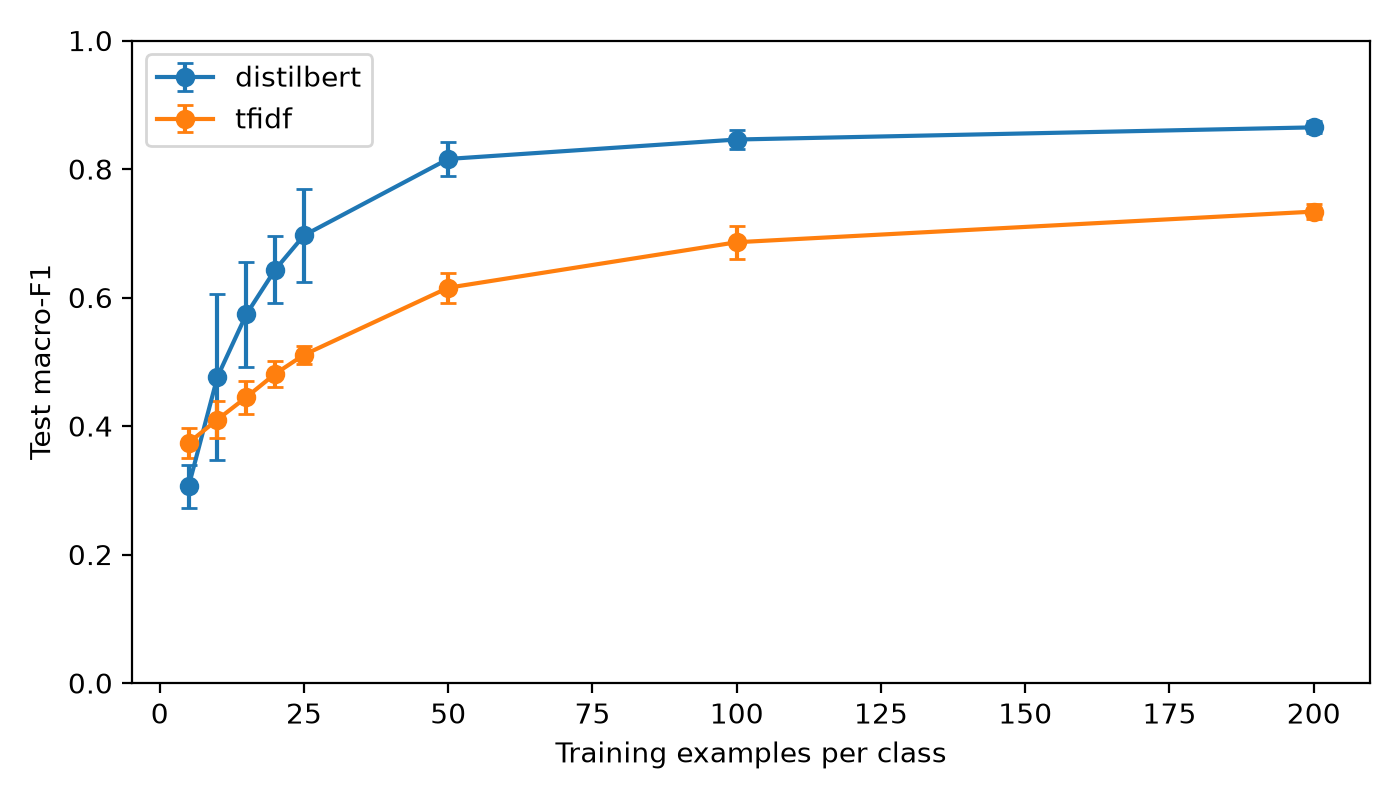
\includegraphics[width=.88\linewidth]{../results/learning_curve.png}
  \caption{Test macro-F1 as the number of training examples increases. Points
  show the mean over three seeds and error bars show one sample standard
  deviation.}
  \label{fig:curve}
\end{figure}

Figure~\ref{fig:curve} shows the learning curves for both models. DistilBERT is
unstable in the 10--25-example range. For example, at 20 examples its three
macro-F1 scores are .651, .691, and .588. The curve begins
to flatten after 50 examples: its mean improves by .030 from 50 to 100 and .019
from 100 to 200. TF--IDF continues to improve, so the absolute gap narrows
after its maximum at 50 examples.

At 200 examples per class, mean measured training
time is 1.23 seconds for TF--IDF and 69.30 seconds for DistilBERT, about 57 times
longer. The corresponding gain is .131 macro-F1.

\section{Discussion, error analysis, and limitations}

Pretraining does eventually give a large advantage, but it does not make DistilBERT the best choice with extremely few
examples per class. A plausible explanation is that TF--IDF can use a few direct
lexical cues immediately, whereas DistilBERT must adapt a newly initialized
classification head as well as its encoder. Ten epochs correspond to only 30
optimizer steps in the five-example condition. At 10--20 examples, the large
between-seed variation agrees with earlier observations that few-sample
fine-tuning can be unstable \citep{zhang2020revisiting}.

At 200 examples per class, DistilBERT's mean per-class F1 scores are .919 for
joy, .871 for anger, .850 for sadness, and .820 for fear. TF--IDF scores .803,
.737, .697, and .698 respectively. DistilBERT therefore performs better on every class. Its most frequent remaining errors, aggregated over
the three runs, are sadness predicted as fear (27 cases), anger as sadness (26),
and anger as fear (21).

Table~\ref{tab:errors} gives three examples from the 200-example runs. In particular, ``I am unconcerned'' has little evidence
for the annotated sadness label when removed from its original conversation.
This is better viewed as annotation or context ambiguity.

\begin{table}[ht]
  \centering
  \caption{Selected test examples. Predictions summarize the three seeds. A
  slash indicates that seeds produced different labels.}
  \label{tab:errors}
  \small
  \begin{tabular}{p{.48\linewidth}lll}
    \toprule
    Comment & Label & TF--IDF & DistilBERT \\
    \midrule
    ``Sun is out, feels great.'' & Joy & Sadness/fear & Joy \\
    ``I don't feel so financially secure.'' & Fear & Sadness & Sadness \\
    ``I am unconcerned.'' & Sadness & Joy/fear & Fear \\
    \bottomrule
  \end{tabular}
\end{table}

Several limitations restrict the conclusion. Only four emotions and
single-label comments are considered, so the task is easier than
the original GoEmotions benchmark. Results may not transfer from Reddit to
other domains. Three seeds expose substantial instability but are too few for
strong statistical claims. The fixed ten-epoch schedule is controlled but may
be unsuitable at the extremes: very small samples receive few optimizer steps,
while larger samples may begin to overfit. A validation-based early-stopping
rule would address this. The models also differ in parameter count and
pretraining cost, which is not included in the runtime comparison. Finally,
manual error analysis is necessarily subjective and the evaluation treats the
dataset labels as ground truth despite clear ambiguous cases.

Useful follow-up experiments would repeat the comparison with more seeds,
compare full fine-tuning with a frozen DistilBERT encoder, and test whether
early stopping reduces low-data variance. A multilabel version would be more
faithful to emotion co-occurrence, but would introduce threshold selection and
different metrics.

\section{Conclusion}

With five labelled examples per emotion, TF--IDF is both better and much cheaper. DistilBERT is
better on average from 10 examples onward, but its results remain strongly
seed-dependent at the smallest sizes. At 15 examples per class it beats TF--IDF
for every test seed, and at 50 examples the advantage is large: .816 versus .615
macro-F1. Improvements after 100 examples are small. For this dataset and
training procedure, 15 examples per class are therefore enough for a consistent
advantage, while roughly 50 are needed for a clear gain.

\clearpage
\bibliographystyle{plainnat}
\bibliography{references}

\section*{Declaration of AI Usage}

I used OpenAI Codex to brainstorm the research question, assist with parts of
the implementation and debugging, and suggest revisions to the report text.
AI assistance substantially influenced portions of the experimental code and
wording. I inspected and modified all generated code, ran the experiments,
checked the reported values against the saved results, and reviewed the final
text and cited claims for correctness. I remain responsible for all submitted
code, analysis, and text.

\end{document}
